\documentclass[1p]{elsarticle_modified}
%\bibliographystyle{elsarticle-num}

%\usepackage[colorlinks]{hyperref}
%\usepackage{abbrmath_seonhwa} %\Abb, \Ascr, \Acal ,\Abf, \Afrak
\usepackage{amsfonts}
\usepackage{amssymb}
\usepackage{amsmath}
\usepackage{amsthm}
\usepackage{scalefnt}
\usepackage{amsbsy}
\usepackage{kotex}
\usepackage{caption}
\usepackage{subfig}
\usepackage{color}
\usepackage{graphicx}
\usepackage{xcolor} %% white, black, red, green, blue, cyan, magenta, yellow
\usepackage{float}
\usepackage{setspace}
\usepackage{hyperref}

\usepackage{tikz}
\usetikzlibrary{arrows}

\usepackage{multirow}
\usepackage{array} % fixed length table
\usepackage{hhline}

%%%%%%%%%%%%%%%%%%%%%
\makeatletter
\renewcommand*\env@matrix[1][\arraystretch]{%
	\edef\arraystretch{#1}%
	\hskip -\arraycolsep
	\let\@ifnextchar\new@ifnextchar
	\array{*\c@MaxMatrixCols c}}
\makeatother %https://tex.stackexchange.com/questions/14071/how-can-i-increase-the-line-spacing-in-a-matrix
%%%%%%%%%%%%%%%

\usepackage[normalem]{ulem}

\newcommand{\msout}[1]{\ifmmode\text{\sout{\ensuremath{#1}}}\else\sout{#1}\fi}
%SOURCE: \msout is \stkout macro in https://tex.stackexchange.com/questions/20609/strikeout-in-math-mode

\newcommand{\cancel}[1]{
	\ifmmode
	{\color{red}\msout{#1}}
	\else
	{\color{red}\sout{#1}}
	\fi
}

\newcommand{\add}[1]{
	{\color{blue}\uwave{#1}}
}

\newcommand{\replace}[2]{
	\ifmmode
	{\color{red}\msout{#1}}{\color{blue}\uwave{#2}}
	\else
	{\color{red}\sout{#1}}{\color{blue}\uwave{#2}}
	\fi
}

\newcommand{\Sol}{\mathcal{S}} %segment
\newcommand{\D}{D} %diagram
\newcommand{\A}{\mathcal{A}} %arc


%%%%%%%%%%%%%%%%%%%%%%%%%%%%%5 test

\def\sl{\operatorname{\textup{SL}}(2,\Cbb)}
\def\psl{\operatorname{\textup{PSL}}(2,\Cbb)}
\def\quan{\mkern 1mu \triangleright \mkern 1mu}

\theoremstyle{definition}
\newtheorem{thm}{Theorem}[section]
\newtheorem{prop}[thm]{Proposition}
\newtheorem{lem}[thm]{Lemma}
\newtheorem{ques}[thm]{Question}
\newtheorem{cor}[thm]{Corollary}
\newtheorem{defn}[thm]{Definition}
\newtheorem{exam}[thm]{Example}
\newtheorem{rmk}[thm]{Remark}
\newtheorem{alg}[thm]{Algorithm}

\newcommand{\I}{\sqrt{-1}}
\begin{document}

%\begin{frontmatter}
%
%\title{Boundary parabolic representations of knots up to 8 crossings}
%
%%% Group authors per affiliation:
%\author{Yunhi Cho} 
%\address{Department of Mathematics, University of Seoul, Seoul, Korea}
%\ead{yhcho@uos.ac.kr}
%
%
%\author{Seonhwa Kim} %\fnref{s_kim}}
%\address{Center for Geometry and Physics, Institute for Basic Science, Pohang, 37673, Korea}
%\ead{ryeona17@ibs.re.kr}
%
%\author{Hyuk Kim}
%\address{Department of Mathematical Sciences, Seoul National University, Seoul 08826, Korea}
%\ead{hyukkim@snu.ac.kr}
%
%\author{Seokbeom Yoon}
%\address{Department of Mathematical Sciences, Seoul National University, Seoul, 08826,  Korea}
%\ead{sbyoon15@snu.ac.kr}
%
%\begin{abstract}
%We find all boundary parabolic representation of knots up to 8 crossings.
%
%\end{abstract}
%\begin{keyword}
%    \MSC[2010] 57M25 
%\end{keyword}
%
%\end{frontmatter}

%\linenumbers
%\tableofcontents
%
\newcommand\colored[1]{\textcolor{white}{\rule[-0.35ex]{0.8em}{1.4ex}}\kern-0.8em\color{red} #1}%
%\newcommand\colored[1]{\textcolor{white}{ #1}\kern-2.17ex	\textcolor{white}{ #1}\kern-1.81ex	\textcolor{white}{ #1}\kern-2.15ex\color{red}#1	}

{\Large $\underline{12n_{0201}~(K12n_{0201})}$}

\setlength{\tabcolsep}{10pt}
\renewcommand{\arraystretch}{1.6}
\vspace{1cm}\begin{tabular}{m{100pt}>{\centering\arraybackslash}m{274pt}}
\multirow{5}{120pt}{
	\centering
	\includegraphics[width=112pt]{../../../GIT/diagram.site/Diagrams/png/2290_12n_0201.png}\\
\ \ \ A knot diagram\footnotemark}&
\allowdisplaybreaks
\textbf{Linearized knot diagam} \\
\cline{2-2}
 &
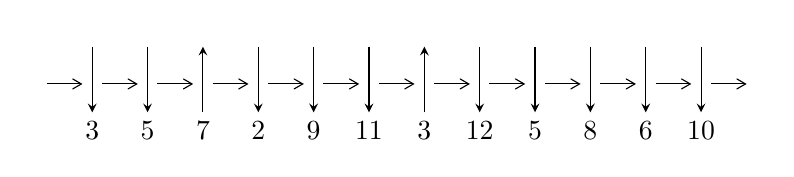
\begin{tikzpicture}[x=20pt, y=17pt]
	% nodes
	\node (C0) at (0, 0) {};
	\node (C1) at (1, 0) {};
	\node (C1U) at (1, +1) {};
	\node (C1D) at (1, -1) {3};

	\node (C2) at (2, 0) {};
	\node (C2U) at (2, +1) {};
	\node (C2D) at (2, -1) {5};

	\node (C3) at (3, 0) {};
	\node (C3U) at (3, +1) {};
	\node (C3D) at (3, -1) {7};

	\node (C4) at (4, 0) {};
	\node (C4U) at (4, +1) {};
	\node (C4D) at (4, -1) {2};

	\node (C5) at (5, 0) {};
	\node (C5U) at (5, +1) {};
	\node (C5D) at (5, -1) {9};

	\node (C6) at (6, 0) {};
	\node (C6U) at (6, +1) {};
	\node (C6D) at (6, -1) {11};

	\node (C7) at (7, 0) {};
	\node (C7U) at (7, +1) {};
	\node (C7D) at (7, -1) {3};

	\node (C8) at (8, 0) {};
	\node (C8U) at (8, +1) {};
	\node (C8D) at (8, -1) {12};

	\node (C9) at (9, 0) {};
	\node (C9U) at (9, +1) {};
	\node (C9D) at (9, -1) {5};

	\node (C10) at (10, 0) {};
	\node (C10U) at (10, +1) {};
	\node (C10D) at (10, -1) {8};

	\node (C11) at (11, 0) {};
	\node (C11U) at (11, +1) {};
	\node (C11D) at (11, -1) {6};

	\node (C12) at (12, 0) {};
	\node (C12U) at (12, +1) {};
	\node (C12D) at (12, -1) {10};
	\node (C13) at (13, 0) {};

	% arrows
	\draw[->,>={angle 60}]
	(C0) edge (C1) (C1) edge (C2) (C2) edge (C3) (C3) edge (C4) (C4) edge (C5) (C5) edge (C6) (C6) edge (C7) (C7) edge (C8) (C8) edge (C9) (C9) edge (C10) (C10) edge (C11) (C11) edge (C12) (C12) edge (C13) ;	\draw[->,>=stealth]
	(C1U) edge (C1D) (C2U) edge (C2D) (C3D) edge (C3U) (C4U) edge (C4D) (C5U) edge (C5D) (C6U) edge (C6D) (C7D) edge (C7U) (C8U) edge (C8D) (C9U) edge (C9D) (C10U) edge (C10D) (C11U) edge (C11D) (C12U) edge (C12D) ;
	\end{tikzpicture} \\
\hhline{~~} \\& 
\textbf{Solving Sequence} \\ \cline{2-2} 
 &
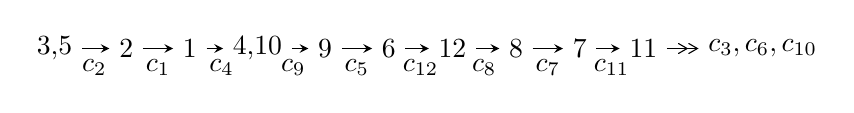
\begin{tikzpicture}[x=23pt, y=7pt]
	% node
	\node (A0) at (-1/8, 0) {3,5};
	\node (A1) at (1, 0) {2};
	\node (A2) at (2, 0) {1};
	\node (A3) at (49/16, 0) {4,10};
	\node (A4) at (33/8, 0) {9};
	\node (A5) at (41/8, 0) {6};
	\node (A6) at (49/8, 0) {12};
	\node (A7) at (57/8, 0) {8};
	\node (A8) at (65/8, 0) {7};
	\node (A9) at (73/8, 0) {11};
	\node (C1) at (1/2, -1) {$c_{2}$};
	\node (C2) at (3/2, -1) {$c_{1}$};
	\node (C3) at (5/2, -1) {$c_{4}$};
	\node (C4) at (29/8, -1) {$c_{9}$};
	\node (C5) at (37/8, -1) {$c_{5}$};
	\node (C6) at (45/8, -1) {$c_{12}$};
	\node (C7) at (53/8, -1) {$c_{8}$};
	\node (C8) at (61/8, -1) {$c_{7}$};
	\node (C9) at (69/8, -1) {$c_{11}$};
	\node (A10) at (11, 0) {$c_{3},c_{6},c_{10}$};

	% edge
	\draw[->,>=stealth]	
	(A0) edge (A1) (A1) edge (A2) (A2) edge (A3) (A3) edge (A4) (A4) edge (A5) (A5) edge (A6) (A6) edge (A7) (A7) edge (A8) (A8) edge (A9) ;
	\draw[->>,>={angle 60}]	
	(A9) edge (A10);
\end{tikzpicture} \\ 

\end{tabular} \\

\footnotetext{
The image of knot diagram is generated by the software ``\textbf{Draw programme}" developed by Andrew Bartholomew(\url{http://www.layer8.co.uk/maths/draw/index.htm\#Running-draw}), where we modified some parts for our purpose(\url{https://github.com/CATsTAILs/LinksPainter}).
}\phantom \\ \newline 
\centering \textbf{Ideals for irreducible components\footnotemark of $X_{\text{par}}$} 
 
\begin{align*}
I^u_{1}&=\langle 
5.14997\times10^{27} u^{29}+1.82430\times10^{28} u^{28}+\cdots+1.93982\times10^{29} b+5.49324\times10^{27},\\
\phantom{I^u_{1}}&\phantom{= \langle  }4.70210\times10^{29} u^{29}+1.55178\times10^{30} u^{28}+\cdots+1.61005\times10^{31} a+6.19868\times10^{31},\\
\phantom{I^u_{1}}&\phantom{= \langle  }u^{30}+5 u^{29}+\cdots-172 u-16\rangle \\
I^u_{2}&=\langle 
-5 u^4 a^3-6 u^4 a^2+\cdots-20 a+39,\;6 u^4 a^2+6 u^4 a+\cdots+5 a-50,\;u^5+u^4-3 u^3-2 u^2+2 u-1\rangle \\
I^u_{3}&=\langle 
- u^{14}-5 u^{13}-6 u^{12}+9 u^{11}+26 u^{10}+10 u^9-21 u^8-15 u^7+6 u^6-7 u^5-19 u^4+2 u^3+15 u^2+b+3 u-3,\\
\phantom{I^u_{3}}&\phantom{= \langle  }3 u^{14}+15 u^{13}+\cdots+a+3,\\
\phantom{I^u_{3}}&\phantom{= \langle  }u^{15}+5 u^{14}+6 u^{13}-9 u^{12}-25 u^{11}-7 u^{10}+22 u^9+10 u^8-11 u^7+7 u^6+18 u^5-6 u^4-15 u^3+4 u-1\rangle \\
I^u_{4}&=\langle 
a^2+2 b- a+2,\;a^3+2 a+1,\;u-1\rangle \\
I^u_{5}&=\langle 
-13 u^5 a^3-13 u^5 a^2+\cdots+a+2,\;u^5 a^3-3 u^5 a^2+\cdots-31 a+33,\;u^6+u^5-2 u^4+2 u^2-2 u-1\rangle \\
I^u_{6}&=\langle 
- a^3+b-2 a+1,\;a^4- a^3+2 a^2-2 a+1,\;u-1\rangle \\
\\
\end{align*}
\raggedright * 6 irreducible components of $\dim_{\mathbb{C}}=0$, with total 96 representations.\\
\footnotetext{All coefficients of polynomials are rational numbers. But the coefficients are sometimes approximated in decimal forms when there is not enough margin.}
\newpage
\renewcommand{\arraystretch}{1}
\centering \section*{I. $I^u_{1}= \langle 5.15\times10^{27} u^{29}+1.82\times10^{28} u^{28}+\cdots+1.94\times10^{29} b+5.49\times10^{27},\;4.70\times10^{29} u^{29}+1.55\times10^{30} u^{28}+\cdots+1.61\times10^{31} a+6.20\times10^{31},\;u^{30}+5 u^{29}+\cdots-172 u-16 \rangle$}
\flushleft \textbf{(i) Arc colorings}\\
\begin{tabular}{m{7pt} m{180pt} m{7pt} m{180pt} }
\flushright $a_{3}=$&$\begin{pmatrix}1\\0\end{pmatrix}$ \\
\flushright $a_{5}=$&$\begin{pmatrix}0\\u\end{pmatrix}$ \\
\flushright $a_{2}=$&$\begin{pmatrix}1\\- u^2\end{pmatrix}$ \\
\flushright $a_{1}=$&$\begin{pmatrix}- u^2+1\\- u^2\end{pmatrix}$ \\
\flushright $a_{4}=$&$\begin{pmatrix}u\\- u^3+u\end{pmatrix}$ \\
\flushright $a_{10}=$&$\begin{pmatrix}-0.0292047 u^{29}-0.0963807 u^{28}+\cdots+15.3253 u-3.84999\\-0.0265487 u^{29}-0.0940447 u^{28}+\cdots+5.13027 u-0.0283182\end{pmatrix}$ \\
\flushright $a_{9}=$&$\begin{pmatrix}-0.0292047 u^{29}-0.0963807 u^{28}+\cdots+15.3253 u-3.84999\\0.0239871 u^{29}+0.113617 u^{28}+\cdots-2.94099 u-0.822600\end{pmatrix}$ \\
\flushright $a_{6}=$&$\begin{pmatrix}-0.0333701 u^{29}-0.154719 u^{28}+\cdots+4.11599 u+2.89975\\-0.0107619 u^{29}-0.0419176 u^{28}+\cdots+0.102195 u+0.142700\end{pmatrix}$ \\
\flushright $a_{12}=$&$\begin{pmatrix}0.0442756 u^{29}+0.200796 u^{28}+\cdots-3.91736 u-2.44196\\-0.00562573 u^{29}-0.00670684 u^{28}+\cdots-1.22478 u-0.441173\end{pmatrix}$ \\
\flushright $a_{8}=$&$\begin{pmatrix}0.0525283 u^{29}+0.229276 u^{28}+\cdots+1.10359 u-4.04234\\0.0233792 u^{29}+0.0945798 u^{28}+\cdots+0.173151 u-0.289600\end{pmatrix}$ \\
\flushright $a_{7}=$&$\begin{pmatrix}0.0291491 u^{29}+0.134696 u^{28}+\cdots+0.930435 u-3.75274\\0.0233792 u^{29}+0.0945798 u^{28}+\cdots+0.173151 u-0.289600\end{pmatrix}$ \\
\flushright $a_{11}=$&$\begin{pmatrix}0.168494 u^{29}+0.707380 u^{28}+\cdots-22.8757 u-5.50128\\-0.00570701 u^{29}-0.0157006 u^{28}+\cdots+0.569930 u-0.316142\end{pmatrix}$\\&\end{tabular}
\flushleft \textbf{(ii) Obstruction class $= -1$}\\~\\
\flushleft \textbf{(iii) Cusp Shapes $= -0.406284 u^{29}-1.66706 u^{28}+\cdots+56.3610 u-5.50399$}\\~\\
\newpage\renewcommand{\arraystretch}{1}
\flushleft \textbf{(iv) u-Polynomials at the component}\newline \\
\begin{tabular}{m{50pt}|m{274pt}}
Crossings & \hspace{64pt}u-Polynomials at each crossing \\
\hline $$\begin{aligned}c_{1}\end{aligned}$$&$\begin{aligned}
&u^{30}+27 u^{29}+\cdots+35696 u+256
\end{aligned}$\\
\hline $$\begin{aligned}c_{2},c_{4}\end{aligned}$$&$\begin{aligned}
&u^{30}-5 u^{29}+\cdots+172 u-16
\end{aligned}$\\
\hline $$\begin{aligned}c_{3},c_{7}\end{aligned}$$&$\begin{aligned}
&u^{30}-6 u^{29}+\cdots+736 u+128
\end{aligned}$\\
\hline $$\begin{aligned}c_{5},c_{6},c_{9}\\c_{11}\end{aligned}$$&$\begin{aligned}
&u^{30}+10 u^{28}+\cdots+u-1
\end{aligned}$\\
\hline $$\begin{aligned}c_{8}\end{aligned}$$&$\begin{aligned}
&u^{30}+24 u^{29}+\cdots+34816 u+2048
\end{aligned}$\\
\hline $$\begin{aligned}c_{10},c_{12}\end{aligned}$$&$\begin{aligned}
&u^{30}- u^{29}+\cdots-2 u+1
\end{aligned}$\\
\hline
\end{tabular}\\~\\
\newpage\renewcommand{\arraystretch}{1}
\flushleft \textbf{(v) Riley Polynomials at the component}\newline \\
\begin{tabular}{m{50pt}|m{274pt}}
Crossings & \hspace{64pt}Riley Polynomials at each crossing \\
\hline $$\begin{aligned}c_{1}\end{aligned}$$&$\begin{aligned}
&y^{30}-43 y^{29}+\cdots-1144368896 y+65536
\end{aligned}$\\
\hline $$\begin{aligned}c_{2},c_{4}\end{aligned}$$&$\begin{aligned}
&y^{30}-27 y^{29}+\cdots-35696 y+256
\end{aligned}$\\
\hline $$\begin{aligned}c_{3},c_{7}\end{aligned}$$&$\begin{aligned}
&y^{30}+12 y^{29}+\cdots-289792 y+16384
\end{aligned}$\\
\hline $$\begin{aligned}c_{5},c_{6},c_{9}\\c_{11}\end{aligned}$$&$\begin{aligned}
&y^{30}+20 y^{29}+\cdots-5 y+1
\end{aligned}$\\
\hline $$\begin{aligned}c_{8}\end{aligned}$$&$\begin{aligned}
&y^{30}+12 y^{29}+\cdots-46137344 y+4194304
\end{aligned}$\\
\hline $$\begin{aligned}c_{10},c_{12}\end{aligned}$$&$\begin{aligned}
&y^{30}-23 y^{29}+\cdots-40 y+1
\end{aligned}$\\
\hline
\end{tabular}\\~\\
\newpage\flushleft \textbf{(vi) Complex Volumes and Cusp Shapes}
$$\begin{array}{c|c|c}  
\text{Solutions to }I^u_{1}& \I (\text{vol} + \sqrt{-1}CS) & \text{Cusp shape}\\
 \hline 
\begin{aligned}
u &= \phantom{-}0.185580 + 0.944093 I \\
a &= -1.001730 + 0.055927 I \\
b &= -1.130640 - 0.094807 I\end{aligned}
 & -0.96646 - 3.13608 I & -4.74984 + 4.49793 I \\ \hline\begin{aligned}
u &= \phantom{-}0.185580 - 0.944093 I \\
a &= -1.001730 - 0.055927 I \\
b &= -1.130640 + 0.094807 I\end{aligned}
 & -0.96646 + 3.13608 I & -4.74984 - 4.49793 I \\ \hline\begin{aligned}
u &= \phantom{-}1.09059\phantom{ +0.000000I} \\
a &= -0.312198\phantom{ +0.000000I} \\
b &= -1.15451\phantom{ +0.000000I}\end{aligned}
 & -2.10768\phantom{ +0.000000I} & \phantom{-}1.10790\phantom{ +0.000000I} \\ \hline\begin{aligned}
u &= -0.640861 + 0.910736 I \\
a &= \phantom{-}0.987047 - 0.263529 I \\
b &= \phantom{-}0.763609 - 0.165945 I\end{aligned}
 & \phantom{-}6.62408 + 4.56917 I & -5.77654 - 9.05645 I \\ \hline\begin{aligned}
u &= -0.640861 - 0.910736 I \\
a &= \phantom{-}0.987047 + 0.263529 I \\
b &= \phantom{-}0.763609 + 0.165945 I\end{aligned}
 & \phantom{-}6.62408 - 4.56917 I & -5.77654 + 9.05645 I \\ \hline\begin{aligned}
u &= \phantom{-}0.412058 + 1.046100 I \\
a &= \phantom{-}1.320550 - 0.089510 I \\
b &= \phantom{-}1.142840 + 0.316503 I\end{aligned}
 & \phantom{-}2.28381 - 11.34220 I & -5.85157 + 7.46971 I \\ \hline\begin{aligned}
u &= \phantom{-}0.412058 - 1.046100 I \\
a &= \phantom{-}1.320550 + 0.089510 I \\
b &= \phantom{-}1.142840 - 0.316503 I\end{aligned}
 & \phantom{-}2.28381 + 11.34220 I & -5.85157 - 7.46971 I \\ \hline\begin{aligned}
u &= -0.858059 + 0.076225 I \\
a &= \phantom{-}0.40465 - 1.62711 I \\
b &= \phantom{-}0.221594 - 0.481448 I\end{aligned}
 & \phantom{-}8.06685 + 5.26278 I & \phantom{-}9.69455 - 9.24591 I \\ \hline\begin{aligned}
u &= -0.858059 - 0.076225 I \\
a &= \phantom{-}0.40465 + 1.62711 I \\
b &= \phantom{-}0.221594 + 0.481448 I\end{aligned}
 & \phantom{-}8.06685 - 5.26278 I & \phantom{-}9.69455 + 9.24591 I \\ \hline\begin{aligned}
u &= \phantom{-}0.697419 + 0.488961 I \\
a &= -0.219398 + 0.713511 I \\
b &= -0.189158 - 0.686223 I\end{aligned}
 & -3.18199 - 1.29456 I & -12.77780 - 2.70196 I\\
 \hline 
 \end{array}$$\newpage$$\begin{array}{c|c|c}  
\text{Solutions to }I^u_{1}& \I (\text{vol} + \sqrt{-1}CS) & \text{Cusp shape}\\
 \hline 
\begin{aligned}
u &= \phantom{-}0.697419 - 0.488961 I \\
a &= -0.219398 - 0.713511 I \\
b &= -0.189158 + 0.686223 I\end{aligned}
 & -3.18199 + 1.29456 I & -12.77780 + 2.70196 I \\ \hline\begin{aligned}
u &= -0.980322 + 0.821398 I \\
a &= -0.268522 + 0.673529 I \\
b &= -0.414628 + 0.219363 I\end{aligned}
 & \phantom{-}5.73142 + 1.70454 I & -14.08727 - 0.46304 I \\ \hline\begin{aligned}
u &= -0.980322 - 0.821398 I \\
a &= -0.268522 - 0.673529 I \\
b &= -0.414628 - 0.219363 I\end{aligned}
 & \phantom{-}5.73142 - 1.70454 I & -14.08727 + 0.46304 I \\ \hline\begin{aligned}
u &= \phantom{-}0.983080 + 0.840486 I \\
a &= -0.207226 - 0.993870 I \\
b &= -0.217086 - 0.194262 I\end{aligned}
 & \phantom{-}0.63688 + 4.93892 I & -8.17431 - 4.19554 I \\ \hline\begin{aligned}
u &= \phantom{-}0.983080 - 0.840486 I \\
a &= -0.207226 + 0.993870 I \\
b &= -0.217086 + 0.194262 I\end{aligned}
 & \phantom{-}0.63688 - 4.93892 I & -8.17431 + 4.19554 I \\ \hline\begin{aligned}
u &= \phantom{-}0.529897 + 0.387033 I \\
a &= \phantom{-}0.760579 + 0.099172 I \\
b &= \phantom{-}0.272048 - 0.498030 I\end{aligned}
 & -0.616430 - 1.153860 I & -7.46498 + 5.62168 I \\ \hline\begin{aligned}
u &= \phantom{-}0.529897 - 0.387033 I \\
a &= \phantom{-}0.760579 - 0.099172 I \\
b &= \phantom{-}0.272048 + 0.498030 I\end{aligned}
 & -0.616430 + 1.153860 I & -7.46498 - 5.62168 I \\ \hline\begin{aligned}
u &= \phantom{-}1.329220 + 0.243682 I \\
a &= \phantom{-}0.323500 + 0.469369 I \\
b &= \phantom{-}1.88537 - 0.37732 I\end{aligned}
 & -4.25514 - 1.03783 I & -6.94488 + 3.56711 I \\ \hline\begin{aligned}
u &= \phantom{-}1.329220 - 0.243682 I \\
a &= \phantom{-}0.323500 - 0.469369 I \\
b &= \phantom{-}1.88537 + 0.37732 I\end{aligned}
 & -4.25514 + 1.03783 I & -6.94488 - 3.56711 I \\ \hline\begin{aligned}
u &= -1.46779 + 0.42678 I \\
a &= \phantom{-}0.428034 - 0.659397 I \\
b &= \phantom{-}1.77991 - 0.18253 I\end{aligned}
 & -6.26616 + 8.18280 I & -7.69035 - 5.49765 I\\
 \hline 
 \end{array}$$\newpage$$\begin{array}{c|c|c}  
\text{Solutions to }I^u_{1}& \I (\text{vol} + \sqrt{-1}CS) & \text{Cusp shape}\\
 \hline 
\begin{aligned}
u &= -1.46779 - 0.42678 I \\
a &= \phantom{-}0.428034 + 0.659397 I \\
b &= \phantom{-}1.77991 + 0.18253 I\end{aligned}
 & -6.26616 - 8.18280 I & -7.69035 + 5.49765 I \\ \hline\begin{aligned}
u &= -1.57146 + 0.14677 I \\
a &= \phantom{-}0.578643 + 0.350914 I \\
b &= \phantom{-}2.02947 + 0.31224 I\end{aligned}
 & -10.76200 + 3.67525 I & -12.88309 - 1.54091 I \\ \hline\begin{aligned}
u &= -1.57146 - 0.14677 I \\
a &= \phantom{-}0.578643 - 0.350914 I \\
b &= \phantom{-}2.02947 - 0.31224 I\end{aligned}
 & -10.76200 - 3.67525 I & -12.88309 + 1.54091 I \\ \hline\begin{aligned}
u &= \phantom{-}1.56632 + 0.22150 I \\
a &= -0.528754 - 0.726360 I \\
b &= -1.94785 - 0.95867 I\end{aligned}
 & -0.77063 - 8.39049 I & -8.00000 + 5.59781 I \\ \hline\begin{aligned}
u &= \phantom{-}1.56632 - 0.22150 I \\
a &= -0.528754 + 0.726360 I \\
b &= -1.94785 + 0.95867 I\end{aligned}
 & -0.77063 + 8.39049 I & -8.00000 - 5.59781 I \\ \hline\begin{aligned}
u &= -1.54411 + 0.40410 I \\
a &= -0.646501 + 0.789954 I \\
b &= -2.35333 + 0.65826 I\end{aligned}
 & -3.9951 + 16.5974 I & -8.00000 - 7.96952 I \\ \hline\begin{aligned}
u &= -1.54411 - 0.40410 I \\
a &= -0.646501 - 0.789954 I \\
b &= -2.35333 - 0.65826 I\end{aligned}
 & -3.9951 - 16.5974 I & -8.00000 + 7.96952 I \\ \hline\begin{aligned}
u &= -1.64278 + 0.07145 I \\
a &= -0.548824 - 0.489947 I \\
b &= -1.50370 - 0.48413 I\end{aligned}
 & -9.12603 - 2.01137 I & -11.51571 + 3.04989 I \\ \hline\begin{aligned}
u &= -1.64278 - 0.07145 I \\
a &= -0.548824 + 0.489947 I \\
b &= -1.50370 + 0.48413 I\end{aligned}
 & -9.12603 + 2.01137 I & -11.51571 - 3.04989 I \\ \hline\begin{aligned}
u &= -0.0869836\phantom{ +0.000000I} \\
a &= -5.20191\phantom{ +0.000000I} \\
b &= -0.522412\phantom{ +0.000000I}\end{aligned}
 & -0.887138\phantom{ +0.000000I} & -11.1170\phantom{ +0.000000I}\\
 \hline 
 \end{array}$$\newpage\newpage\renewcommand{\arraystretch}{1}
\centering \section*{II. $I^u_{2}= \langle -5 u^4 a^3-6 u^4 a^2+\cdots-20 a+39,\;6 u^4 a^2+6 u^4 a+\cdots+5 a-50,\;u^5+u^4-3 u^3-2 u^2+2 u-1 \rangle$}
\flushleft \textbf{(i) Arc colorings}\\
\begin{tabular}{m{7pt} m{180pt} m{7pt} m{180pt} }
\flushright $a_{3}=$&$\begin{pmatrix}1\\0\end{pmatrix}$ \\
\flushright $a_{5}=$&$\begin{pmatrix}0\\u\end{pmatrix}$ \\
\flushright $a_{2}=$&$\begin{pmatrix}1\\- u^2\end{pmatrix}$ \\
\flushright $a_{1}=$&$\begin{pmatrix}- u^2+1\\- u^2\end{pmatrix}$ \\
\flushright $a_{4}=$&$\begin{pmatrix}u\\- u^3+u\end{pmatrix}$ \\
\flushright $a_{10}=$&$\begin{pmatrix}a\\0.172414 a^{3} u^{4}+0.206897 a^{2} u^{4}+\cdots+0.689655 a-1.34483\end{pmatrix}$ \\
\flushright $a_{9}=$&$\begin{pmatrix}a\\0.172414 a^{3} u^{4}+0.206897 a^{2} u^{4}+\cdots+0.689655 a-1.34483\end{pmatrix}$ \\
\flushright $a_{6}=$&$\begin{pmatrix}- a^2 u\\-0.448276 a^{3} u^{4}-1.13793 a^{2} u^{4}+\cdots+0.206897 a+0.896552\end{pmatrix}$ \\
\flushright $a_{12}=$&$\begin{pmatrix}-0.206897 a^{3} u^{4}-0.448276 a^{2} u^{4}+\cdots+1.17241 a+4.41379\\-0.551724 a^{3} u^{4}-0.862069 a^{2} u^{4}+\cdots+0.793103 a+3.10345\end{pmatrix}$ \\
\flushright $a_{8}=$&$\begin{pmatrix}-1\\- u^3+2 u-1\end{pmatrix}$ \\
\flushright $a_{7}=$&$\begin{pmatrix}u^3-2 u\\- u^3+2 u-1\end{pmatrix}$ \\
\flushright $a_{11}=$&$\begin{pmatrix}-0.172414 a^{3} u^{4}-0.206897 a^{2} u^{4}+\cdots+1.31034 a+1.34483\\-0.310345 a^{3} u^{4}-0.172414 a^{2} u^{4}+\cdots-0.241379 a-1.37931\end{pmatrix}$\\&\end{tabular}
\flushleft \textbf{(ii) Obstruction class $= -1$}\\~\\
\flushleft \textbf{(iii) Cusp Shapes $= -\frac{20}{29} u^4 a^3-\frac{24}{29} u^4 a^2+\cdots+\frac{36}{29} a-\frac{18}{29}$}\\~\\
\newpage\renewcommand{\arraystretch}{1}
\flushleft \textbf{(iv) u-Polynomials at the component}\newline \\
\begin{tabular}{m{50pt}|m{274pt}}
Crossings & \hspace{64pt}u-Polynomials at each crossing \\
\hline $$\begin{aligned}c_{1}\end{aligned}$$&$\begin{aligned}
&(u^5+7 u^4+17 u^3+14 u^2+1)^4
\end{aligned}$\\
\hline $$\begin{aligned}c_{2},c_{4}\end{aligned}$$&$\begin{aligned}
&(u^5- u^4-3 u^3+2 u^2+2 u+1)^4
\end{aligned}$\\
\hline $$\begin{aligned}c_{3},c_{7}\end{aligned}$$&$\begin{aligned}
&(u^5+3 u^4+6 u^3+7 u^2+4 u+2)^4
\end{aligned}$\\
\hline $$\begin{aligned}c_{5},c_{6},c_{9}\\c_{11}\end{aligned}$$&$\begin{aligned}
&u^{20}+u^{19}+\cdots-88 u+43
\end{aligned}$\\
\hline $$\begin{aligned}c_{8}\end{aligned}$$&$\begin{aligned}
&(u^2- u+1)^{10}
\end{aligned}$\\
\hline $$\begin{aligned}c_{10},c_{12}\end{aligned}$$&$\begin{aligned}
&u^{20}-3 u^{19}+\cdots-204 u+61
\end{aligned}$\\
\hline
\end{tabular}\\~\\
\newpage\renewcommand{\arraystretch}{1}
\flushleft \textbf{(v) Riley Polynomials at the component}\newline \\
\begin{tabular}{m{50pt}|m{274pt}}
Crossings & \hspace{64pt}Riley Polynomials at each crossing \\
\hline $$\begin{aligned}c_{1}\end{aligned}$$&$\begin{aligned}
&(y^5-15 y^4+93 y^3-210 y^2-28 y-1)^4
\end{aligned}$\\
\hline $$\begin{aligned}c_{2},c_{4}\end{aligned}$$&$\begin{aligned}
&(y^5-7 y^4+17 y^3-14 y^2-1)^4
\end{aligned}$\\
\hline $$\begin{aligned}c_{3},c_{7}\end{aligned}$$&$\begin{aligned}
&(y^5+3 y^4+2 y^3-13 y^2-12 y-4)^4
\end{aligned}$\\
\hline $$\begin{aligned}c_{5},c_{6},c_{9}\\c_{11}\end{aligned}$$&$\begin{aligned}
&y^{20}+9 y^{19}+\cdots+8424 y+1849
\end{aligned}$\\
\hline $$\begin{aligned}c_{8}\end{aligned}$$&$\begin{aligned}
&(y^2+y+1)^{10}
\end{aligned}$\\
\hline $$\begin{aligned}c_{10},c_{12}\end{aligned}$$&$\begin{aligned}
&y^{20}-7 y^{19}+\cdots+49640 y+3721
\end{aligned}$\\
\hline
\end{tabular}\\~\\
\newpage\flushleft \textbf{(vi) Complex Volumes and Cusp Shapes}
$$\begin{array}{c|c|c}  
\text{Solutions to }I^u_{2}& \I (\text{vol} + \sqrt{-1}CS) & \text{Cusp shape}\\
 \hline 
\begin{aligned}
u &= \phantom{-}0.331409 + 0.386277 I \\
a &= \phantom{-}1.34411 + 1.58943 I \\
b &= \phantom{-}1.46009 + 0.56077 I\end{aligned}
 & \phantom{-}4.56162 + 0.89106 I & -2.71808 + 2.59039 I \\ \hline\begin{aligned}
u &= \phantom{-}0.331409 + 0.386277 I \\
a &= \phantom{-}2.21697 + 1.44611 I \\
b &= \phantom{-}1.55827 - 1.58798 I\end{aligned}
 & \phantom{-}4.56162 - 3.16871 I & -2.71808 + 9.51860 I \\ \hline\begin{aligned}
u &= \phantom{-}0.331409 + 0.386277 I \\
a &= -2.71697 - 0.58008 I \\
b &= -0.264187 + 0.240329 I\end{aligned}
 & \phantom{-}4.56162 - 3.16871 I & -2.71808 + 9.51860 I \\ \hline\begin{aligned}
u &= \phantom{-}0.331409 + 0.386277 I \\
a &= -1.84411 - 2.45545 I \\
b &= -0.94003 + 1.23377 I\end{aligned}
 & \phantom{-}4.56162 + 0.89106 I & -2.71808 + 2.59039 I \\ \hline\begin{aligned}
u &= \phantom{-}0.331409 - 0.386277 I \\
a &= \phantom{-}1.34411 - 1.58943 I \\
b &= \phantom{-}1.46009 - 0.56077 I\end{aligned}
 & \phantom{-}4.56162 - 0.89106 I & -2.71808 - 2.59039 I \\ \hline\begin{aligned}
u &= \phantom{-}0.331409 - 0.386277 I \\
a &= \phantom{-}2.21697 - 1.44611 I \\
b &= \phantom{-}1.55827 + 1.58798 I\end{aligned}
 & \phantom{-}4.56162 + 3.16871 I & -2.71808 - 9.51860 I \\ \hline\begin{aligned}
u &= \phantom{-}0.331409 - 0.386277 I \\
a &= -2.71697 + 0.58008 I \\
b &= -0.264187 - 0.240329 I\end{aligned}
 & \phantom{-}4.56162 + 3.16871 I & -2.71808 - 9.51860 I \\ \hline\begin{aligned}
u &= \phantom{-}0.331409 - 0.386277 I \\
a &= -1.84411 + 2.45545 I \\
b &= -0.94003 - 1.23377 I\end{aligned}
 & \phantom{-}4.56162 - 0.89106 I & -2.71808 - 2.59039 I \\ \hline\begin{aligned}
u &= \phantom{-}1.49784\phantom{ +0.000000I} \\
a &= -0.736571 + 0.258832 I \\
b &= -2.15778 + 0.06792 I\end{aligned}
 & -3.58001 - 2.02988 I & -8.28576 + 3.46410 I \\ \hline\begin{aligned}
u &= \phantom{-}1.49784\phantom{ +0.000000I} \\
a &= -0.736571 - 0.258832 I \\
b &= -2.15778 - 0.06792 I\end{aligned}
 & -3.58001 + 2.02988 I & -8.28576 - 3.46410 I\\
 \hline 
 \end{array}$$\newpage$$\begin{array}{c|c|c}  
\text{Solutions to }I^u_{2}& \I (\text{vol} + \sqrt{-1}CS) & \text{Cusp shape}\\
 \hline 
\begin{aligned}
u &= \phantom{-}1.49784\phantom{ +0.000000I} \\
a &= \phantom{-}0.236571 + 0.607193 I \\
b &= \phantom{-}1.35362 + 1.32492 I\end{aligned}
 & -3.58001 - 2.02988 I & -8.28576 + 3.46410 I \\ \hline\begin{aligned}
u &= \phantom{-}1.49784\phantom{ +0.000000I} \\
a &= \phantom{-}0.236571 - 0.607193 I \\
b &= \phantom{-}1.35362 - 1.32492 I\end{aligned}
 & -3.58001 + 2.02988 I & -8.28576 - 3.46410 I \\ \hline\begin{aligned}
u &= -1.58033 + 0.28256 I \\
a &= -0.950991 - 0.218765 I \\
b &= -2.22328 - 0.39754 I\end{aligned}
 & -8.52888 + 9.02707 I & -9.13904 - 7.01094 I \\ \hline\begin{aligned}
u &= -1.58033 + 0.28256 I \\
a &= -0.723737 + 0.541697 I \\
b &= -2.02311 + 0.30398 I\end{aligned}
 & -8.52888 + 4.96731 I & -9.13904 - 0.08273 I \\ \hline\begin{aligned}
u &= -1.58033 + 0.28256 I \\
a &= \phantom{-}0.450991 - 0.647260 I \\
b &= \phantom{-}2.26931 - 0.79527 I\end{aligned}
 & -8.52888 + 9.02707 I & -9.13904 - 7.01094 I \\ \hline\begin{aligned}
u &= -1.58033 + 0.28256 I \\
a &= \phantom{-}0.223737 + 0.324328 I \\
b &= \phantom{-}0.967085 + 0.252556 I\end{aligned}
 & -8.52888 + 4.96731 I & -9.13904 - 0.08273 I \\ \hline\begin{aligned}
u &= -1.58033 - 0.28256 I \\
a &= -0.950991 + 0.218765 I \\
b &= -2.22328 + 0.39754 I\end{aligned}
 & -8.52888 - 9.02707 I & -9.13904 + 7.01094 I \\ \hline\begin{aligned}
u &= -1.58033 - 0.28256 I \\
a &= -0.723737 - 0.541697 I \\
b &= -2.02311 - 0.30398 I\end{aligned}
 & -8.52888 - 4.96731 I & -9.13904 + 0.08273 I \\ \hline\begin{aligned}
u &= -1.58033 - 0.28256 I \\
a &= \phantom{-}0.450991 + 0.647260 I \\
b &= \phantom{-}2.26931 + 0.79527 I\end{aligned}
 & -8.52888 - 9.02707 I & -9.13904 + 7.01094 I \\ \hline\begin{aligned}
u &= -1.58033 - 0.28256 I \\
a &= \phantom{-}0.223737 - 0.324328 I \\
b &= \phantom{-}0.967085 - 0.252556 I\end{aligned}
 & -8.52888 - 4.96731 I & -9.13904 + 0.08273 I\\
 \hline 
 \end{array}$$\newpage\newpage\renewcommand{\arraystretch}{1}
\centering \section*{III. $I^u_{3}= \langle - u^{14}-5 u^{13}+\cdots+b-3,\;3 u^{14}+15 u^{13}+\cdots+a+3,\;u^{15}+5 u^{14}+\cdots+4 u-1 \rangle$}
\flushleft \textbf{(i) Arc colorings}\\
\begin{tabular}{m{7pt} m{180pt} m{7pt} m{180pt} }
\flushright $a_{3}=$&$\begin{pmatrix}1\\0\end{pmatrix}$ \\
\flushright $a_{5}=$&$\begin{pmatrix}0\\u\end{pmatrix}$ \\
\flushright $a_{2}=$&$\begin{pmatrix}1\\- u^2\end{pmatrix}$ \\
\flushright $a_{1}=$&$\begin{pmatrix}- u^2+1\\- u^2\end{pmatrix}$ \\
\flushright $a_{4}=$&$\begin{pmatrix}u\\- u^3+u\end{pmatrix}$ \\
\flushright $a_{10}=$&$\begin{pmatrix}-3 u^{14}-15 u^{13}+\cdots+10 u-3\\u^{14}+5 u^{13}+\cdots-3 u+3\end{pmatrix}$ \\
\flushright $a_{9}=$&$\begin{pmatrix}-3 u^{14}-15 u^{13}+\cdots+10 u-3\\3 u^{14}+13 u^{13}+\cdots-24 u^2+3\end{pmatrix}$ \\
\flushright $a_{6}=$&$\begin{pmatrix}4 u^{14}+19 u^{13}+\cdots-5 u+9\\2 u^{14}+11 u^{13}+\cdots-7 u^2-7 u\end{pmatrix}$ \\
\flushright $a_{12}=$&$\begin{pmatrix}u^{12}+4 u^{11}+3 u^{10}-8 u^9-14 u^8- u^7+9 u^6-2 u^4+9 u^3+6 u^2-4 u-3\\-2 u^{14}-7 u^{13}+\cdots+16 u^2-3 u\end{pmatrix}$ \\
\flushright $a_{8}=$&$\begin{pmatrix}- u^{12}-3 u^{11}+\cdots+4 u-1\\2 u^{14}+8 u^{13}+\cdots-8 u^2+3 u\end{pmatrix}$ \\
\flushright $a_{7}=$&$\begin{pmatrix}-2 u^{14}-8 u^{13}+\cdots+u-1\\2 u^{14}+8 u^{13}+\cdots-8 u^2+3 u\end{pmatrix}$ \\
\flushright $a_{11}=$&$\begin{pmatrix}-3 u^{14}-15 u^{13}+\cdots+10 u-2\\2 u^{14}+9 u^{13}+\cdots-3 u+3\end{pmatrix}$\\&\end{tabular}
\flushleft \textbf{(ii) Obstruction class $= 1$}\\~\\
\flushleft \textbf{(iii) Cusp Shapes $= 3 u^{14}+15 u^{13}+23 u^{12}-4 u^{11}-48 u^{10}-46 u^9-7 u^8-4 u^7-21 u^6+4 u^5+30 u^4+16 u^3-4 u^2- u-3$}\\~\\
\newpage\renewcommand{\arraystretch}{1}
\flushleft \textbf{(iv) u-Polynomials at the component}\newline \\
\begin{tabular}{m{50pt}|m{274pt}}
Crossings & \hspace{64pt}u-Polynomials at each crossing \\
\hline $$\begin{aligned}c_{1}\end{aligned}$$&$\begin{aligned}
&u^{15}-13 u^{14}+\cdots+16 u-1
\end{aligned}$\\
\hline $$\begin{aligned}c_{2}\end{aligned}$$&$\begin{aligned}
&u^{15}+5 u^{14}+\cdots+4 u-1
\end{aligned}$\\
\hline $$\begin{aligned}c_{3}\end{aligned}$$&$\begin{aligned}
&u^{15}- u^{14}+\cdots-8 u^2-1
\end{aligned}$\\
\hline $$\begin{aligned}c_{4}\end{aligned}$$&$\begin{aligned}
&u^{15}-5 u^{14}+\cdots+4 u+1
\end{aligned}$\\
\hline $$\begin{aligned}c_{5},c_{11}\end{aligned}$$&$\begin{aligned}
&u^{15}+7 u^{13}+\cdots- u+1
\end{aligned}$\\
\hline $$\begin{aligned}c_{6},c_{9}\end{aligned}$$&$\begin{aligned}
&u^{15}+7 u^{13}+\cdots- u-1
\end{aligned}$\\
\hline $$\begin{aligned}c_{7}\end{aligned}$$&$\begin{aligned}
&u^{15}+u^{14}+\cdots+8 u^2+1
\end{aligned}$\\
\hline $$\begin{aligned}c_{8}\end{aligned}$$&$\begin{aligned}
&u^{15}+5 u^{13}+\cdots+u-1
\end{aligned}$\\
\hline $$\begin{aligned}c_{10},c_{12}\end{aligned}$$&$\begin{aligned}
&u^{15}+u^{14}+\cdots+5 u^2+1
\end{aligned}$\\
\hline
\end{tabular}\\~\\
\newpage\renewcommand{\arraystretch}{1}
\flushleft \textbf{(v) Riley Polynomials at the component}\newline \\
\begin{tabular}{m{50pt}|m{274pt}}
Crossings & \hspace{64pt}Riley Polynomials at each crossing \\
\hline $$\begin{aligned}c_{1}\end{aligned}$$&$\begin{aligned}
&y^{15}-17 y^{14}+\cdots-8 y-1
\end{aligned}$\\
\hline $$\begin{aligned}c_{2},c_{4}\end{aligned}$$&$\begin{aligned}
&y^{15}-13 y^{14}+\cdots+16 y-1
\end{aligned}$\\
\hline $$\begin{aligned}c_{3},c_{7}\end{aligned}$$&$\begin{aligned}
&y^{15}+3 y^{14}+\cdots-16 y-1
\end{aligned}$\\
\hline $$\begin{aligned}c_{5},c_{6},c_{9}\\c_{11}\end{aligned}$$&$\begin{aligned}
&y^{15}+14 y^{14}+\cdots+3 y-1
\end{aligned}$\\
\hline $$\begin{aligned}c_{8}\end{aligned}$$&$\begin{aligned}
&y^{15}+10 y^{14}+\cdots+y-1
\end{aligned}$\\
\hline $$\begin{aligned}c_{10},c_{12}\end{aligned}$$&$\begin{aligned}
&y^{15}- y^{14}+\cdots-10 y-1
\end{aligned}$\\
\hline
\end{tabular}\\~\\
\newpage\flushleft \textbf{(vi) Complex Volumes and Cusp Shapes}
$$\begin{array}{c|c|c}  
\text{Solutions to }I^u_{3}& \I (\text{vol} + \sqrt{-1}CS) & \text{Cusp shape}\\
 \hline 
\begin{aligned}
u &= -0.796754 + 0.693348 I \\
a &= -0.847137 + 0.671365 I \\
b &= -0.497650 - 0.022952 I\end{aligned}
 & \phantom{-}6.79252 + 3.72902 I & -3.12247 - 0.91109 I \\ \hline\begin{aligned}
u &= -0.796754 - 0.693348 I \\
a &= -0.847137 - 0.671365 I \\
b &= -0.497650 + 0.022952 I\end{aligned}
 & \phantom{-}6.79252 - 3.72902 I & -3.12247 + 0.91109 I \\ \hline\begin{aligned}
u &= \phantom{-}0.930890 + 0.056485 I \\
a &= -0.285629 + 1.354480 I \\
b &= \phantom{-}4.78949 + 1.58588 I\end{aligned}
 & \phantom{-}3.42636 + 1.92079 I & -18.2159 - 15.3647 I \\ \hline\begin{aligned}
u &= \phantom{-}0.930890 - 0.056485 I \\
a &= -0.285629 - 1.354480 I \\
b &= \phantom{-}4.78949 - 1.58588 I\end{aligned}
 & \phantom{-}3.42636 - 1.92079 I & -18.2159 + 15.3647 I \\ \hline\begin{aligned}
u &= \phantom{-}0.401039 + 0.815529 I \\
a &= -0.507179 + 0.227656 I \\
b &= -0.692924 - 0.171185 I\end{aligned}
 & -2.12132 - 2.26307 I & -9.68770 + 3.58355 I \\ \hline\begin{aligned}
u &= \phantom{-}0.401039 - 0.815529 I \\
a &= -0.507179 - 0.227656 I \\
b &= -0.692924 + 0.171185 I\end{aligned}
 & -2.12132 + 2.26307 I & -9.68770 - 3.58355 I \\ \hline\begin{aligned}
u &= -0.989330 + 0.711734 I \\
a &= \phantom{-}0.287415 - 0.801453 I \\
b &= \phantom{-}0.343746 - 0.514545 I\end{aligned}
 & \phantom{-}6.20548 + 1.67451 I & \phantom{-}3.16227 - 0.38526 I \\ \hline\begin{aligned}
u &= -0.989330 - 0.711734 I \\
a &= \phantom{-}0.287415 + 0.801453 I \\
b &= \phantom{-}0.343746 + 0.514545 I\end{aligned}
 & \phantom{-}6.20548 - 1.67451 I & \phantom{-}3.16227 + 0.38526 I \\ \hline\begin{aligned}
u &= \phantom{-}1.36474\phantom{ +0.000000I} \\
a &= \phantom{-}0.285599\phantom{ +0.000000I} \\
b &= \phantom{-}1.95225\phantom{ +0.000000I}\end{aligned}
 & -4.46149\phantom{ +0.000000I} & -9.01920\phantom{ +0.000000I} \\ \hline\begin{aligned}
u &= -1.46931 + 0.07528 I \\
a &= -0.353185 + 1.029040 I \\
b &= -1.57621 + 0.50876 I\end{aligned}
 & -1.37277 + 3.16303 I & -7.59589 - 1.64203 I\\
 \hline 
 \end{array}$$\newpage$$\begin{array}{c|c|c}  
\text{Solutions to }I^u_{3}& \I (\text{vol} + \sqrt{-1}CS) & \text{Cusp shape}\\
 \hline 
\begin{aligned}
u &= -1.46931 - 0.07528 I \\
a &= -0.353185 - 1.029040 I \\
b &= -1.57621 - 0.50876 I\end{aligned}
 & -1.37277 - 3.16303 I & -7.59589 + 1.64203 I \\ \hline\begin{aligned}
u &= -1.56575 + 0.31338 I \\
a &= \phantom{-}0.532385 - 0.260435 I \\
b &= \phantom{-}1.78333 - 0.18434 I\end{aligned}
 & -8.65053 + 6.60987 I & -9.62356 - 4.91898 I \\ \hline\begin{aligned}
u &= -1.56575 - 0.31338 I \\
a &= \phantom{-}0.532385 + 0.260435 I \\
b &= \phantom{-}1.78333 + 0.18434 I\end{aligned}
 & -8.65053 - 6.60987 I & -9.62356 + 4.91898 I \\ \hline\begin{aligned}
u &= \phantom{-}0.306844 + 0.131865 I \\
a &= \phantom{-}2.53053 + 3.22263 I \\
b &= \phantom{-}0.87409 - 1.42027 I\end{aligned}
 & \phantom{-}4.53074 - 2.24627 I & -3.40718 + 0.47377 I \\ \hline\begin{aligned}
u &= \phantom{-}0.306844 - 0.131865 I \\
a &= \phantom{-}2.53053 - 3.22263 I \\
b &= \phantom{-}0.87409 + 1.42027 I\end{aligned}
 & \phantom{-}4.53074 + 2.24627 I & -3.40718 - 0.47377 I\\
 \hline 
 \end{array}$$\newpage\newpage\renewcommand{\arraystretch}{1}
\centering \section*{IV. $I^u_{4}= \langle a^2+2 b- a+2,\;a^3+2 a+1,\;u-1 \rangle$}
\flushleft \textbf{(i) Arc colorings}\\
\begin{tabular}{m{7pt} m{180pt} m{7pt} m{180pt} }
\flushright $a_{3}=$&$\begin{pmatrix}1\\0\end{pmatrix}$ \\
\flushright $a_{5}=$&$\begin{pmatrix}0\\1\end{pmatrix}$ \\
\flushright $a_{2}=$&$\begin{pmatrix}1\\-1\end{pmatrix}$ \\
\flushright $a_{1}=$&$\begin{pmatrix}0\\-1\end{pmatrix}$ \\
\flushright $a_{4}=$&$\begin{pmatrix}1\\0\end{pmatrix}$ \\
\flushright $a_{10}=$&$\begin{pmatrix}a\\-\frac{1}{2} a^2+\frac{1}{2} a-1\end{pmatrix}$ \\
\flushright $a_{9}=$&$\begin{pmatrix}a\\-\frac{1}{2} a^2-\frac{1}{2} a-1\end{pmatrix}$ \\
\flushright $a_{6}=$&$\begin{pmatrix}- a^2\\\frac{1}{2} a^2+\frac{1}{2}\end{pmatrix}$ \\
\flushright $a_{12}=$&$\begin{pmatrix}- a^2\\-\frac{1}{2} a^2-\frac{3}{2}\end{pmatrix}$ \\
\flushright $a_{8}=$&$\begin{pmatrix}a^2- a-1\\0\end{pmatrix}$ \\
\flushright $a_{7}=$&$\begin{pmatrix}a^2- a-1\\0\end{pmatrix}$ \\
\flushright $a_{11}=$&$\begin{pmatrix}- a^2-2 a-1\\-\frac{1}{2} a^2+\frac{1}{2} a-1\end{pmatrix}$\\&\end{tabular}
\flushleft \textbf{(ii) Obstruction class $= 1$}\\~\\
\flushleft \textbf{(iii) Cusp Shapes $= -\frac{17}{4} a^2+\frac{1}{2} a-\frac{97}{4}$}\\~\\
\newpage\renewcommand{\arraystretch}{1}
\flushleft \textbf{(iv) u-Polynomials at the component}\newline \\
\begin{tabular}{m{50pt}|m{274pt}}
Crossings & \hspace{64pt}u-Polynomials at each crossing \\
\hline $$\begin{aligned}c_{1},c_{2}\end{aligned}$$&$\begin{aligned}
&(u-1)^3
\end{aligned}$\\
\hline $$\begin{aligned}c_{3},c_{7}\end{aligned}$$&$\begin{aligned}
&u^3
\end{aligned}$\\
\hline $$\begin{aligned}c_{4}\end{aligned}$$&$\begin{aligned}
&(u+1)^3
\end{aligned}$\\
\hline $$\begin{aligned}c_{5},c_{6}\end{aligned}$$&$\begin{aligned}
&u^3+2 u-1
\end{aligned}$\\
\hline $$\begin{aligned}c_{8}\end{aligned}$$&$\begin{aligned}
&u^3-3 u^2+5 u-2
\end{aligned}$\\
\hline $$\begin{aligned}c_{9},c_{10},c_{11}\\c_{12}\end{aligned}$$&$\begin{aligned}
&u^3+2 u+1
\end{aligned}$\\
\hline
\end{tabular}\\~\\
\newpage\renewcommand{\arraystretch}{1}
\flushleft \textbf{(v) Riley Polynomials at the component}\newline \\
\begin{tabular}{m{50pt}|m{274pt}}
Crossings & \hspace{64pt}Riley Polynomials at each crossing \\
\hline $$\begin{aligned}c_{1},c_{2},c_{4}\end{aligned}$$&$\begin{aligned}
&(y-1)^3
\end{aligned}$\\
\hline $$\begin{aligned}c_{3},c_{7}\end{aligned}$$&$\begin{aligned}
&y^3
\end{aligned}$\\
\hline $$\begin{aligned}c_{5},c_{6},c_{9}\\c_{10},c_{11},c_{12}\end{aligned}$$&$\begin{aligned}
&y^3+4 y^2+4 y-1
\end{aligned}$\\
\hline $$\begin{aligned}c_{8}\end{aligned}$$&$\begin{aligned}
&y^3+y^2+13 y-4
\end{aligned}$\\
\hline
\end{tabular}\\~\\
\newpage\flushleft \textbf{(vi) Complex Volumes and Cusp Shapes}
$$\begin{array}{c|c|c}  
\text{Solutions to }I^u_{4}& \I (\text{vol} + \sqrt{-1}CS) & \text{Cusp shape}\\
 \hline 
\begin{aligned}
u &= \phantom{-}1.00000\phantom{ +0.000000I} \\
a &= \phantom{-}0.22670 + 1.46771 I \\
b &= \phantom{-}0.164742 + 0.401127 I\end{aligned}
 & \phantom{-}7.79580 - 5.13794 I & -15.1998 - 2.0943 I \\ \hline\begin{aligned}
u &= \phantom{-}1.00000\phantom{ +0.000000I} \\
a &= \phantom{-}0.22670 - 1.46771 I \\
b &= \phantom{-}0.164742 - 0.401127 I\end{aligned}
 & \phantom{-}7.79580 + 5.13794 I & -15.1998 + 2.0943 I \\ \hline\begin{aligned}
u &= \phantom{-}1.00000\phantom{ +0.000000I} \\
a &= -0.453398\phantom{ +0.000000I} \\
b &= -1.32948\phantom{ +0.000000I}\end{aligned}
 & -2.43213\phantom{ +0.000000I} & -25.3500\phantom{ +0.000000I}\\
 \hline 
 \end{array}$$\newpage\newpage\renewcommand{\arraystretch}{1}
\centering \section*{V. $I^u_{5}= \langle -13 u^5 a^3-13 u^5 a^2+\cdots+a+2,\;u^5 a^3-3 u^5 a^2+\cdots-31 a+33,\;u^6+u^5-2 u^4+2 u^2-2 u-1 \rangle$}
\flushleft \textbf{(i) Arc colorings}\\
\begin{tabular}{m{7pt} m{180pt} m{7pt} m{180pt} }
\flushright $a_{3}=$&$\begin{pmatrix}1\\0\end{pmatrix}$ \\
\flushright $a_{5}=$&$\begin{pmatrix}0\\u\end{pmatrix}$ \\
\flushright $a_{2}=$&$\begin{pmatrix}1\\- u^2\end{pmatrix}$ \\
\flushright $a_{1}=$&$\begin{pmatrix}- u^2+1\\- u^2\end{pmatrix}$ \\
\flushright $a_{4}=$&$\begin{pmatrix}u\\- u^3+u\end{pmatrix}$ \\
\flushright $a_{10}=$&$\begin{pmatrix}a\\1.18182 a^{3} u^{5}+1.18182 a^{2} u^{5}+\cdots-0.0909091 a-0.181818\end{pmatrix}$ \\
\flushright $a_{9}=$&$\begin{pmatrix}a\\1.18182 a^{3} u^{5}+1.18182 a^{2} u^{5}+\cdots-0.0909091 a-0.181818\end{pmatrix}$ \\
\flushright $a_{6}=$&$\begin{pmatrix}- a^2 u\\0.909091 a^{3} u^{5}-1.09091 a^{2} u^{5}+\cdots-0.454545 a+1.09091\end{pmatrix}$ \\
\flushright $a_{12}=$&$\begin{pmatrix}1.09091 a^{3} u^{5}-0.909091 a^{2} u^{5}+\cdots-0.545455 a+2.90909\\-2.45455 a^{3} u^{5}-2.45455 a^{2} u^{5}+\cdots+0.727273 a-0.545455\end{pmatrix}$ \\
\flushright $a_{8}=$&$\begin{pmatrix}- u^5+2 u^3-2 u^2- u+3\\u^5- u^3+u^2- u\end{pmatrix}$ \\
\flushright $a_{7}=$&$\begin{pmatrix}-2 u^5+3 u^3-3 u^2+3\\u^5- u^3+u^2- u\end{pmatrix}$ \\
\flushright $a_{11}=$&$\begin{pmatrix}0.454545 a^{3} u^{5}-0.545455 a^{2} u^{5}+\cdots-2.72727 a+5.54545\\-0.181818 a^{3} u^{5}+0.818182 a^{2} u^{5}+\cdots+0.0909091 a+0.181818\end{pmatrix}$\\&\end{tabular}
\flushleft \textbf{(ii) Obstruction class $= -1$}\\~\\
\flushleft \textbf{(iii) Cusp Shapes $= \frac{4}{11} u^5 a^3+\frac{48}{11} u^5 a^2+\cdots+\frac{20}{11} a-\frac{70}{11}$}\\~\\
\newpage\renewcommand{\arraystretch}{1}
\flushleft \textbf{(iv) u-Polynomials at the component}\newline \\
\begin{tabular}{m{50pt}|m{274pt}}
Crossings & \hspace{64pt}u-Polynomials at each crossing \\
\hline $$\begin{aligned}c_{1}\end{aligned}$$&$\begin{aligned}
&(u^6+5 u^5+8 u^4+6 u^3+8 u^2+8 u+1)^4
\end{aligned}$\\
\hline $$\begin{aligned}c_{2},c_{4}\end{aligned}$$&$\begin{aligned}
&(u^6- u^5-2 u^4+2 u^2+2 u-1)^4
\end{aligned}$\\
\hline $$\begin{aligned}c_{3},c_{7}\end{aligned}$$&$\begin{aligned}
&(u^3- u^2+2 u-1)^8
\end{aligned}$\\
\hline $$\begin{aligned}c_{5},c_{6},c_{9}\\c_{11}\end{aligned}$$&$\begin{aligned}
&u^{24}+u^{23}+\cdots-14 u+67
\end{aligned}$\\
\hline $$\begin{aligned}c_{8}\end{aligned}$$&$\begin{aligned}
&(u^2- u+1)^{12}
\end{aligned}$\\
\hline $$\begin{aligned}c_{10},c_{12}\end{aligned}$$&$\begin{aligned}
&u^{24}-7 u^{23}+\cdots-122 u+61
\end{aligned}$\\
\hline
\end{tabular}\\~\\
\newpage\renewcommand{\arraystretch}{1}
\flushleft \textbf{(v) Riley Polynomials at the component}\newline \\
\begin{tabular}{m{50pt}|m{274pt}}
Crossings & \hspace{64pt}Riley Polynomials at each crossing \\
\hline $$\begin{aligned}c_{1}\end{aligned}$$&$\begin{aligned}
&(y^6-9 y^5+20 y^4+14 y^3-16 y^2-48 y+1)^4
\end{aligned}$\\
\hline $$\begin{aligned}c_{2},c_{4}\end{aligned}$$&$\begin{aligned}
&(y^6-5 y^5+8 y^4-6 y^3+8 y^2-8 y+1)^4
\end{aligned}$\\
\hline $$\begin{aligned}c_{3},c_{7}\end{aligned}$$&$\begin{aligned}
&(y^3+3 y^2+2 y-1)^8
\end{aligned}$\\
\hline $$\begin{aligned}c_{5},c_{6},c_{9}\\c_{11}\end{aligned}$$&$\begin{aligned}
&y^{24}+21 y^{23}+\cdots+24192 y+4489
\end{aligned}$\\
\hline $$\begin{aligned}c_{8}\end{aligned}$$&$\begin{aligned}
&(y^2+y+1)^{12}
\end{aligned}$\\
\hline $$\begin{aligned}c_{10},c_{12}\end{aligned}$$&$\begin{aligned}
&y^{24}+5 y^{23}+\cdots-37820 y+3721
\end{aligned}$\\
\hline
\end{tabular}\\~\\
\newpage\flushleft \textbf{(vi) Complex Volumes and Cusp Shapes}
$$\begin{array}{c|c|c}  
\text{Solutions to }I^u_{5}& \I (\text{vol} + \sqrt{-1}CS) & \text{Cusp shape}\\
 \hline 
\begin{aligned}
u &= \phantom{-}0.592989 + 0.847544 I \\
a &= \phantom{-}0.929183 - 0.410221 I \\
b &= \phantom{-}0.885713 - 0.329153 I\end{aligned}
 & -1.37919 - 0.79824 I & -7.50976 - 0.48465 I \\ \hline\begin{aligned}
u &= \phantom{-}0.592989 + 0.847544 I \\
a &= -1.026620 - 0.271921 I \\
b &= -0.997939 - 0.570659 I\end{aligned}
 & -1.37919 - 4.85801 I & -7.50976 + 6.44355 I \\ \hline\begin{aligned}
u &= \phantom{-}0.592989 + 0.847544 I \\
a &= \phantom{-}0.515331 - 1.058190 I \\
b &= \phantom{-}0.1116080 - 0.0764541 I\end{aligned}
 & -1.37919 - 4.85801 I & -7.50976 + 6.44355 I \\ \hline\begin{aligned}
u &= \phantom{-}0.592989 + 0.847544 I \\
a &= \phantom{-}0.478377 + 0.632485 I \\
b &= \phantom{-}0.117869 - 0.114876 I\end{aligned}
 & -1.37919 - 0.79824 I & -7.50976 - 0.48465 I \\ \hline\begin{aligned}
u &= \phantom{-}0.592989 - 0.847544 I \\
a &= \phantom{-}0.929183 + 0.410221 I \\
b &= \phantom{-}0.885713 + 0.329153 I\end{aligned}
 & -1.37919 + 0.79824 I & -7.50976 + 0.48465 I \\ \hline\begin{aligned}
u &= \phantom{-}0.592989 - 0.847544 I \\
a &= -1.026620 + 0.271921 I \\
b &= -0.997939 + 0.570659 I\end{aligned}
 & -1.37919 + 4.85801 I & -7.50976 - 6.44355 I \\ \hline\begin{aligned}
u &= \phantom{-}0.592989 - 0.847544 I \\
a &= \phantom{-}0.515331 + 1.058190 I \\
b &= \phantom{-}0.1116080 + 0.0764541 I\end{aligned}
 & -1.37919 + 4.85801 I & -7.50976 - 6.44355 I \\ \hline\begin{aligned}
u &= \phantom{-}0.592989 - 0.847544 I \\
a &= \phantom{-}0.478377 - 0.632485 I \\
b &= \phantom{-}0.117869 + 0.114876 I\end{aligned}
 & -1.37919 + 0.79824 I & -7.50976 + 0.48465 I \\ \hline\begin{aligned}
u &= \phantom{-}1.13416\phantom{ +0.000000I} \\
a &= \phantom{-}0.385031 + 0.931825 I \\
b &= -0.34379 + 5.37612 I\end{aligned}
 & \phantom{-}2.75839 - 2.02988 I & -0.98049 + 3.46410 I \\ \hline\begin{aligned}
u &= \phantom{-}1.13416\phantom{ +0.000000I} \\
a &= \phantom{-}0.385031 - 0.931825 I \\
b &= -0.34379 - 5.37612 I\end{aligned}
 & \phantom{-}2.75839 + 2.02988 I & -0.98049 - 3.46410 I\\
 \hline 
 \end{array}$$\newpage$$\begin{array}{c|c|c}  
\text{Solutions to }I^u_{5}& \I (\text{vol} + \sqrt{-1}CS) & \text{Cusp shape}\\
 \hline 
\begin{aligned}
u &= \phantom{-}1.13416\phantom{ +0.000000I} \\
a &= -0.217824 + 1.221440 I \\
b &= -2.14651 + 1.06279 I\end{aligned}
 & \phantom{-}2.75839 + 2.02988 I & -0.98049 - 3.46410 I \\ \hline\begin{aligned}
u &= \phantom{-}1.13416\phantom{ +0.000000I} \\
a &= -0.217824 - 1.221440 I \\
b &= -2.14651 - 1.06279 I\end{aligned}
 & \phantom{-}2.75839 - 2.02988 I & -0.98049 + 3.46410 I \\ \hline\begin{aligned}
u &= -1.47043 + 0.10268 I \\
a &= -0.155430 + 0.985327 I \\
b &= -0.719608 - 0.619193 I\end{aligned}
 & -1.37919 + 4.85801 I & -7.50976 - 6.44355 I \\ \hline\begin{aligned}
u &= -1.47043 + 0.10268 I \\
a &= \phantom{-}0.848595 - 0.875871 I \\
b &= \phantom{-}2.24219 - 1.17501 I\end{aligned}
 & -1.37919 + 4.85801 I & -7.50976 - 6.44355 I \\ \hline\begin{aligned}
u &= -1.47043 + 0.10268 I \\
a &= -0.074026 - 1.295000 I \\
b &= -0.039244 - 1.020410 I\end{aligned}
 & -1.37919 + 0.79824 I & -7.50976 + 0.48465 I \\ \hline\begin{aligned}
u &= -1.47043 + 0.10268 I \\
a &= -0.177765 + 0.639970 I \\
b &= -2.27588 + 0.59891 I\end{aligned}
 & -1.37919 + 0.79824 I & -7.50976 + 0.48465 I \\ \hline\begin{aligned}
u &= -1.47043 - 0.10268 I \\
a &= -0.155430 - 0.985327 I \\
b &= -0.719608 + 0.619193 I\end{aligned}
 & -1.37919 - 4.85801 I & -7.50976 + 6.44355 I \\ \hline\begin{aligned}
u &= -1.47043 - 0.10268 I \\
a &= \phantom{-}0.848595 + 0.875871 I \\
b &= \phantom{-}2.24219 + 1.17501 I\end{aligned}
 & -1.37919 - 4.85801 I & -7.50976 + 6.44355 I \\ \hline\begin{aligned}
u &= -1.47043 - 0.10268 I \\
a &= -0.074026 + 1.295000 I \\
b &= -0.039244 + 1.020410 I\end{aligned}
 & -1.37919 - 0.79824 I & -7.50976 - 0.48465 I \\ \hline\begin{aligned}
u &= -1.47043 - 0.10268 I \\
a &= -0.177765 - 0.639970 I \\
b &= -2.27588 - 0.59891 I\end{aligned}
 & -1.37919 - 0.79824 I & -7.50976 - 0.48465 I\\
 \hline 
 \end{array}$$\newpage$$\begin{array}{c|c|c}  
\text{Solutions to }I^u_{5}& \I (\text{vol} + \sqrt{-1}CS) & \text{Cusp shape}\\
 \hline 
\begin{aligned}
u &= -0.379278\phantom{ +0.000000I} \\
a &= \phantom{-}1.80591 + 0.63475 I \\
b &= \phantom{-}0.436714 + 0.501880 I\end{aligned}
 & \phantom{-}2.75839 - 2.02988 I & -0.98049 + 3.46410 I \\ \hline\begin{aligned}
u &= -0.379278\phantom{ +0.000000I} \\
a &= \phantom{-}1.80591 - 0.63475 I \\
b &= \phantom{-}0.436714 - 0.501880 I\end{aligned}
 & \phantom{-}2.75839 + 2.02988 I & -0.98049 - 3.46410 I \\ \hline\begin{aligned}
u &= -0.379278\phantom{ +0.000000I} \\
a &= -0.31076 + 3.22443 I \\
b &= -0.271129 + 0.788683 I\end{aligned}
 & \phantom{-}2.75839 + 2.02988 I & -0.98049 - 3.46410 I \\ \hline\begin{aligned}
u &= -0.379278\phantom{ +0.000000I} \\
a &= -0.31076 - 3.22443 I \\
b &= -0.271129 - 0.788683 I\end{aligned}
 & \phantom{-}2.75839 - 2.02988 I & -0.98049 + 3.46410 I\\
 \hline 
 \end{array}$$\newpage\newpage\renewcommand{\arraystretch}{1}
\centering \section*{VI. $I^u_{6}= \langle - a^3+b-2 a+1,\;a^4- a^3+2 a^2-2 a+1,\;u-1 \rangle$}
\flushleft \textbf{(i) Arc colorings}\\
\begin{tabular}{m{7pt} m{180pt} m{7pt} m{180pt} }
\flushright $a_{3}=$&$\begin{pmatrix}1\\0\end{pmatrix}$ \\
\flushright $a_{5}=$&$\begin{pmatrix}0\\1\end{pmatrix}$ \\
\flushright $a_{2}=$&$\begin{pmatrix}1\\-1\end{pmatrix}$ \\
\flushright $a_{1}=$&$\begin{pmatrix}0\\-1\end{pmatrix}$ \\
\flushright $a_{4}=$&$\begin{pmatrix}1\\0\end{pmatrix}$ \\
\flushright $a_{10}=$&$\begin{pmatrix}a\\a^3+2 a-1\end{pmatrix}$ \\
\flushright $a_{9}=$&$\begin{pmatrix}a\\a^3+a-1\end{pmatrix}$ \\
\flushright $a_{6}=$&$\begin{pmatrix}- a^2\\- a^3+a^2- a+2\end{pmatrix}$ \\
\flushright $a_{12}=$&$\begin{pmatrix}- a^2\\- a^3- a\end{pmatrix}$ \\
\flushright $a_{8}=$&$\begin{pmatrix}1\\0\end{pmatrix}$ \\
\flushright $a_{7}=$&$\begin{pmatrix}1\\0\end{pmatrix}$ \\
\flushright $a_{11}=$&$\begin{pmatrix}- a^3- a+1\\a^3+2 a-1\end{pmatrix}$\\&\end{tabular}
\flushleft \textbf{(ii) Obstruction class $= 1$}\\~\\
\flushleft \textbf{(iii) Cusp Shapes $= 4 a^3+4 a-12$}\\~\\
\newpage\renewcommand{\arraystretch}{1}
\flushleft \textbf{(iv) u-Polynomials at the component}\newline \\
\begin{tabular}{m{50pt}|m{274pt}}
Crossings & \hspace{64pt}u-Polynomials at each crossing \\
\hline $$\begin{aligned}c_{1},c_{2}\end{aligned}$$&$\begin{aligned}
&(u-1)^4
\end{aligned}$\\
\hline $$\begin{aligned}c_{3},c_{7}\end{aligned}$$&$\begin{aligned}
&u^4
\end{aligned}$\\
\hline $$\begin{aligned}c_{4}\end{aligned}$$&$\begin{aligned}
&(u+1)^4
\end{aligned}$\\
\hline $$\begin{aligned}c_{5},c_{6}\end{aligned}$$&$\begin{aligned}
&u^4+u^3+2 u^2+2 u+1
\end{aligned}$\\
\hline $$\begin{aligned}c_{8}\end{aligned}$$&$\begin{aligned}
&(u^2+u+1)^2
\end{aligned}$\\
\hline $$\begin{aligned}c_{9},c_{10},c_{11}\\c_{12}\end{aligned}$$&$\begin{aligned}
&u^4- u^3+2 u^2-2 u+1
\end{aligned}$\\
\hline
\end{tabular}\\~\\
\newpage\renewcommand{\arraystretch}{1}
\flushleft \textbf{(v) Riley Polynomials at the component}\newline \\
\begin{tabular}{m{50pt}|m{274pt}}
Crossings & \hspace{64pt}Riley Polynomials at each crossing \\
\hline $$\begin{aligned}c_{1},c_{2},c_{4}\end{aligned}$$&$\begin{aligned}
&(y-1)^4
\end{aligned}$\\
\hline $$\begin{aligned}c_{3},c_{7}\end{aligned}$$&$\begin{aligned}
&y^4
\end{aligned}$\\
\hline $$\begin{aligned}c_{5},c_{6},c_{9}\\c_{10},c_{11},c_{12}\end{aligned}$$&$\begin{aligned}
&y^4+3 y^3+2 y^2+1
\end{aligned}$\\
\hline $$\begin{aligned}c_{8}\end{aligned}$$&$\begin{aligned}
&(y^2+y+1)^2
\end{aligned}$\\
\hline
\end{tabular}\\~\\
\newpage\flushleft \textbf{(vi) Complex Volumes and Cusp Shapes}
$$\begin{array}{c|c|c}  
\text{Solutions to }I^u_{6}& \I (\text{vol} + \sqrt{-1}CS) & \text{Cusp shape}\\
 \hline 
\begin{aligned}
u &= \phantom{-}1.00000\phantom{ +0.000000I} \\
a &= \phantom{-}0.621744 + 0.440597 I \\
b &= \phantom{-}0.121744 + 1.306620 I\end{aligned}
 & \phantom{-}1.64493 - 2.02988 I & -10.00000 + 3.46410 I \\ \hline\begin{aligned}
u &= \phantom{-}1.00000\phantom{ +0.000000I} \\
a &= \phantom{-}0.621744 - 0.440597 I \\
b &= \phantom{-}0.121744 - 1.306620 I\end{aligned}
 & \phantom{-}1.64493 + 2.02988 I & -10.00000 - 3.46410 I \\ \hline\begin{aligned}
u &= \phantom{-}1.00000\phantom{ +0.000000I} \\
a &= -0.121744 + 1.306620 I \\
b &= -0.621744 + 0.440597 I\end{aligned}
 & \phantom{-}1.64493 + 2.02988 I & -10.00000 - 3.46410 I \\ \hline\begin{aligned}
u &= \phantom{-}1.00000\phantom{ +0.000000I} \\
a &= -0.121744 - 1.306620 I \\
b &= -0.621744 - 0.440597 I\end{aligned}
 & \phantom{-}1.64493 - 2.02988 I & -10.00000 + 3.46410 I\\
 \hline 
 \end{array}$$\newpage
\newpage\renewcommand{\arraystretch}{1}
\centering \section*{ VII. u-Polynomials}
\begin{tabular}{m{50pt}|m{274pt}}
Crossings & \hspace{64pt}u-Polynomials at each crossing \\
\hline $$\begin{aligned}c_{1}\end{aligned}$$&$\begin{aligned}
&(u-1)^7(u^5+7 u^4+17 u^3+14 u^2+1)^4\\
&\cdot((u^6+5 u^5+\cdots+8 u+1)^{4})(u^{15}-13 u^{14}+\cdots+16 u-1)\\
&\cdot(u^{30}+27 u^{29}+\cdots+35696 u+256)
\end{aligned}$\\
\hline $$\begin{aligned}c_{2}\end{aligned}$$&$\begin{aligned}
&(u-1)^7(u^5- u^4-3 u^3+2 u^2+2 u+1)^4\\
&\cdot((u^6- u^5-2 u^4+2 u^2+2 u-1)^4)(u^{15}+5 u^{14}+\cdots+4 u-1)\\
&\cdot(u^{30}-5 u^{29}+\cdots+172 u-16)
\end{aligned}$\\
\hline $$\begin{aligned}c_{3}\end{aligned}$$&$\begin{aligned}
&u^7(u^3- u^2+2 u-1)^8(u^5+3 u^4+6 u^3+7 u^2+4 u+2)^4\\
&\cdot(u^{15}- u^{14}+\cdots-8 u^2-1)(u^{30}-6 u^{29}+\cdots+736 u+128)
\end{aligned}$\\
\hline $$\begin{aligned}c_{4}\end{aligned}$$&$\begin{aligned}
&(u+1)^7(u^5- u^4-3 u^3+2 u^2+2 u+1)^4\\
&\cdot((u^6- u^5-2 u^4+2 u^2+2 u-1)^4)(u^{15}-5 u^{14}+\cdots+4 u+1)\\
&\cdot(u^{30}-5 u^{29}+\cdots+172 u-16)
\end{aligned}$\\
\hline $$\begin{aligned}c_{5}\end{aligned}$$&$\begin{aligned}
&(u^3+2 u-1)(u^4+u^3+2 u^2+2 u+1)(u^{15}+7 u^{13}+\cdots- u+1)\\
&\cdot(u^{20}+u^{19}+\cdots-88 u+43)(u^{24}+u^{23}+\cdots-14 u+67)\\
&\cdot(u^{30}+10 u^{28}+\cdots+u-1)
\end{aligned}$\\
\hline $$\begin{aligned}c_{6}\end{aligned}$$&$\begin{aligned}
&(u^3+2 u-1)(u^4+u^3+2 u^2+2 u+1)(u^{15}+7 u^{13}+\cdots- u-1)\\
&\cdot(u^{20}+u^{19}+\cdots-88 u+43)(u^{24}+u^{23}+\cdots-14 u+67)\\
&\cdot(u^{30}+10 u^{28}+\cdots+u-1)
\end{aligned}$\\
\hline $$\begin{aligned}c_{7}\end{aligned}$$&$\begin{aligned}
&u^7(u^3- u^2+2 u-1)^8(u^5+3 u^4+6 u^3+7 u^2+4 u+2)^4\\
&\cdot(u^{15}+u^{14}+\cdots+8 u^2+1)(u^{30}-6 u^{29}+\cdots+736 u+128)
\end{aligned}$\\
\hline $$\begin{aligned}c_{8}\end{aligned}$$&$\begin{aligned}
&((u^2- u+1)^{22})(u^2+u+1)^2(u^{3}-3 u^{2}+5 u-2)(u^{15}+5 u^{13}+\cdots+u-1)\\
&\cdot(u^{30}+24 u^{29}+\cdots+34816 u+2048)
\end{aligned}$\\
\hline $$\begin{aligned}c_{9}\end{aligned}$$&$\begin{aligned}
&(u^3+2 u+1)(u^4- u^3+2 u^2-2 u+1)(u^{15}+7 u^{13}+\cdots- u-1)\\
&\cdot(u^{20}+u^{19}+\cdots-88 u+43)(u^{24}+u^{23}+\cdots-14 u+67)\\
&\cdot(u^{30}+10 u^{28}+\cdots+u-1)
\end{aligned}$\\
\hline $$\begin{aligned}c_{10},c_{12}\end{aligned}$$&$\begin{aligned}
&(u^3+2 u+1)(u^4- u^3+2 u^2-2 u+1)(u^{15}+u^{14}+\cdots+5 u^2+1)\\
&\cdot(u^{20}-3 u^{19}+\cdots-204 u+61)(u^{24}-7 u^{23}+\cdots-122 u+61)\\
&\cdot(u^{30}- u^{29}+\cdots-2 u+1)
\end{aligned}$\\
\hline $$\begin{aligned}c_{11}\end{aligned}$$&$\begin{aligned}
&(u^3+2 u+1)(u^4- u^3+2 u^2-2 u+1)(u^{15}+7 u^{13}+\cdots- u+1)\\
&\cdot(u^{20}+u^{19}+\cdots-88 u+43)(u^{24}+u^{23}+\cdots-14 u+67)\\
&\cdot(u^{30}+10 u^{28}+\cdots+u-1)
\end{aligned}$\\
\hline
\end{tabular}\newpage\renewcommand{\arraystretch}{1}
\centering \section*{ VIII. Riley Polynomials}
\begin{tabular}{m{50pt}|m{274pt}}
Crossings & \hspace{64pt}Riley Polynomials at each crossing \\
\hline $$\begin{aligned}c_{1}\end{aligned}$$&$\begin{aligned}
&(y-1)^7(y^5-15 y^4+93 y^3-210 y^2-28 y-1)^4\\
&\cdot(y^6-9 y^5+20 y^4+14 y^3-16 y^2-48 y+1)^4\\
&\cdot(y^{15}-17 y^{14}+\cdots-8 y-1)\\
&\cdot(y^{30}-43 y^{29}+\cdots-1144368896 y+65536)
\end{aligned}$\\
\hline $$\begin{aligned}c_{2},c_{4}\end{aligned}$$&$\begin{aligned}
&(y-1)^7(y^5-7 y^4+17 y^3-14 y^2-1)^4\\
&\cdot((y^6-5 y^5+\cdots-8 y+1)^{4})(y^{15}-13 y^{14}+\cdots+16 y-1)\\
&\cdot(y^{30}-27 y^{29}+\cdots-35696 y+256)
\end{aligned}$\\
\hline $$\begin{aligned}c_{3},c_{7}\end{aligned}$$&$\begin{aligned}
&y^7(y^3+3 y^2+2 y-1)^8(y^5+3 y^4+2 y^3-13 y^2-12 y-4)^4\\
&\cdot(y^{15}+3 y^{14}+\cdots-16 y-1)(y^{30}+12 y^{29}+\cdots-289792 y+16384)
\end{aligned}$\\
\hline $$\begin{aligned}c_{5},c_{6},c_{9}\\c_{11}\end{aligned}$$&$\begin{aligned}
&(y^3+4 y^2+4 y-1)(y^4+3 y^3+2 y^2+1)(y^{15}+14 y^{14}+\cdots+3 y-1)\\
&\cdot(y^{20}+9 y^{19}+\cdots+8424 y+1849)\\
&\cdot(y^{24}+21 y^{23}+\cdots+24192 y+4489)(y^{30}+20 y^{29}+\cdots-5 y+1)
\end{aligned}$\\
\hline $$\begin{aligned}c_{8}\end{aligned}$$&$\begin{aligned}
&((y^2+y+1)^{24})(y^3+y^2+13 y-4)(y^{15}+10 y^{14}+\cdots+y-1)\\
&\cdot(y^{30}+12 y^{29}+\cdots-46137344 y+4194304)
\end{aligned}$\\
\hline $$\begin{aligned}c_{10},c_{12}\end{aligned}$$&$\begin{aligned}
&(y^3+4 y^2+4 y-1)(y^4+3 y^3+2 y^2+1)(y^{15}- y^{14}+\cdots-10 y-1)\\
&\cdot(y^{20}-7 y^{19}+\cdots+49640 y+3721)\\
&\cdot(y^{24}+5 y^{23}+\cdots-37820 y+3721)(y^{30}-23 y^{29}+\cdots-40 y+1)
\end{aligned}$\\
\hline
\end{tabular}
\vskip 2pc
\end{document}